\documentclass[12pt]{article}
\usepackage[utf8]{inputenc}
\usepackage[T1]{fontenc}
\usepackage[brazil]{babel}
\usepackage{amsmath, amssymb, array, bm, geometry, booktabs, siunitx, graphicx, colortbl, parskip, xcolor}
\usepackage{listings}
\usepackage{color}
\usepackage{float}
\usepackage{fancyhdr}
\usepackage{titlesec}
\usepackage{hyperref}
\usepackage{listings}

\setlength{\headheight}{14.5pt}
\addtolength{\topmargin}{-2.5pt}
\geometry{a4paper, total={6in, 9in}}




\definecolor{codegray}{gray}{0.9}
\lstset{
    backgroundcolor=\color{codegray},
    basicstyle=\ttfamily\footnotesize,
    frame=single,
    breaklines=true,
    captionpos=b,
    numbers=left,
    numberstyle=\tiny,
    language=Python
}

% Cabeçalho
\pagestyle{fancy}
\fancyhf{}
\rhead{UnB}
\lhead{Departamento de Ci\^encias Mec\^anicas}
\cfoot{\thepage}

\titleformat{\section}{\large\bfseries}{\thesection}{1em}{}

\begin{document}

% Capa
\begin{titlepage}
    \centering
    
\includegraphics[width=12cm]{img/unb_bandeira.png} \\
    \vspace{1cm}
    \textsc{\Large Universidade de Bras\'ilia} \\
    \textsc{Departamento de Ciências Mec\^anicas} \\
    \textsc{Programa de P\'os-Gradua\c{c}\~ao} \\
    \vfill
    {\Large\bfseries Programa 5} \\
    \vspace{0.5cm}
    {\Large\bfseries Solução de Problemas Lineares - Estudo de caso} \\
    \vspace{0.5cm}
    \textbf{Disciplina: M\'etodos Num\'ericos} \\
    Professor: Dr. Rafael Gabler Gontijo \\
    \vfill
    \textbf{Aluno: Eng. Lucas Wanick — Mestrando em Engenharia Mec\^anica} \\
    \vspace{0.5cm}
        \today \\
\end{titlepage}


\section{Introdução}
O cálculo das raízes de polinômios reais é um problema clássico da análise numérica, com aplicações em diversas áreas da engenharia. Entre os métodos tradicionais para esta tarefa, o \textbf{Método de Bairstow} destaca-se por sua capacidade de extrair raízes reais e complexas conjugadas a partir de um polinômio com coeficientes reais, sem necessidade de operações sobre números complexos durante o processo iterativo.

O método consiste em fatorar o polinômio original $P(x)$ em fatores quadráticos da forma:

\[
x^2 + rx + s
\]

A cada etapa, o algoritmo ajusta iterativamente os parâmetros $(r, s)$ de modo que o fator extraído aproxime um par de raízes reais ou complexas conjugadas. A partir das raízes do fator quadrático, o polinômio é deflacionado, e o processo se repete até que todas as raízes sejam determinadas.

Apesar de sua eficiência, o Método de Bairstow é sensível às condições iniciais de $(r, s)$, e pode apresentar dificuldades em casos de raízes múltiplas, raízes próximas ou polinômios degenerados. Esta sensibilidade motiva a utilização de uma abordagem de \textit{busca em malha} (grid search), onde diversas combinações iniciais de $(r, s)$ são testadas para mapear a convergência do método.

Curiosamente, o comportamento do Método de Bairstow sobre o espaço de chutes iniciais $(r, s)$ revela padrões fractais — regiões com rápida convergência alternam com regiões de lenta convergência ou não convergência, produzindo figuras complexas e auto-similares. Estes \textbf{fractais de iteração} constituem uma ferramenta visual poderosa para estudar a dinâmica do método.


\section{Descrição do Método}

O Método de Bairstow parte de um polinômio de grau $n$ com coeficientes reais:
\[
P(x) = a_n x^n + a_{n-1} x^{n-1} + \ldots + a_1 x + a_0
\]

Em cada etapa, busca-se dividir $P(x)$ por um fator quadrático proposto:

\[
Q(x) = x^2 + rx + s
\]

resultando em:

\[
P(x) = Q(x) \cdot B(x) + R(x)
\]

onde $B(x)$ é o quociente, e $R(x)$ é o resto, que deve tender a zero para que o fator $Q(x)$ represente um par de raízes válido.

O método utiliza as fórmulas de Bairstow, derivadas da diferenciação do esquema de Horner, para atualizar iterativamente $(r, s)$ até que o resíduo seja menor que uma tolerância pré-definida.

Após a extração de um fator quadrático, o polinômio é deflacionado e o processo prossegue até que seu grau seja reduzido a zero.

\section{Malha de Chutes e Relação com Fractais}

Devido à sensibilidade do método às condições iniciais, implementou-se uma \textbf{malha de chutes} — uma discretização do plano $(r, s)$ — onde para cada ponto $(r, s)$ da malha é realizada uma tentativa completa de fatoração.

Em cada ponto, é registrado o número de iterações acumuladas para extrair todas as raízes. A malha resultante permite construir uma imagem fractal, onde a coloração representa o número de iterações.

Este mapa revela a topologia do espaço de chutes — regiões de estabilidade, de rápida convergência, de comportamento caótico e de não convergência — evidenciando a complexidade dinâmica do Método de Bairstow.

\section{Estruturação do Código}

O código foi estruturado em Python, com foco em modularidade e robustez. As principais escolhas e soluções foram:

\begin{itemize}
\item Controle do número de threads das bibliotecas \texttt{OpenBLAS}, \texttt{MKL} e \texttt{OpenMP} para evitar conflitos e sobrecarga em ambientes multicore;
\item Função \texttt{safe\_input()} para permitir interrupção segura do programa
\item Detecção de polinômios degenerados (coeficientes nulos) com interrupção preventiva
\item Estratégia de fallback linear quando o fator quadrático não converge;
\item Eliminação de loops infinitos via controle refinado das iterações;
\item Registro acumulado do número de iterações, respeitando o comportamento natural do método (cada fator quadrático ou linear contribui com até \texttt{maxit} iterações).
\end{itemize}

O código também implementa rotinas para geração de fractais em escala HSV, exportação de dados e interface interativa com o usuário.

\section{Dificuldades Enfrentadas}

Durante o desenvolvimento, as principais dificuldades enfrentadas foram:

\begin{itemize}
\item Loop infinito causado pelo reinício da contagem de iterações em casos de singularidade no Jacobiano;
\item Sensibilidade extrema do método em polinômios com raízes múltiplas e/ou muito próximas;
\item Necessidade de preservar o mapa de iterações mesmo quando o método não converge (para que o fractal seja informativo);
\item Controle do custo computacional da malha, que cresce com a resolução e o grau do polinômio.
\end{itemize}

Todas essas questões foram superadas com ajustes na lógica de iteração, controle de deflação e validação da convergência.

\section{Custo Computacional}

O custo computacional do método cresce linearmente com o número de pontos da malha $(r,s)$ e com o número de iterações realizadas por ponto.

\[
C \propto N_r \times N_s \times \left(\sum_{\text{raízes}} \text{iter\_count}\right)
\]

O uso de paralelismo (\texttt{joblib}) permite explorar múltiplos núcleos, mas o custo ainda é considerável para polinômios de alto grau e malhas finas. Tipicamente, malhas de $1000 \times 1000$ com polinômios de grau $5$ ou $6$ requerem minutos de execução.,

\section{Exemplos e Resultados}

Foram utilizados diversos polinômios de teste:

\begin{itemize}
\item Grau 3: $x^3 - 6x^2 + 11x - 6$;
\item Grau 4: $x^4 - 10x^3 + 35x^2 - 50x + 24$;
\item Grau 5: $x^5 - 5x^4 + 4x^3 + 22x^2 - 21x - 18$;
\item Grau 6: $x^6 - 3x^4 + 3x^2 - 1$.
\end{itemize}

A seguir, apresentamos alguns dos fractais gerados:

\begin{figure}[H]
\centering
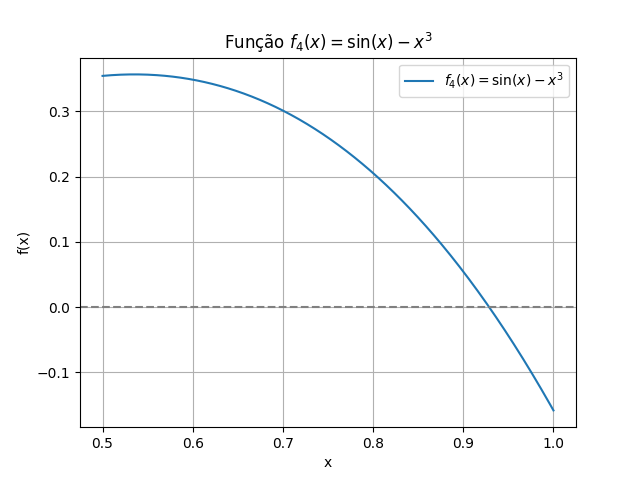
\includegraphics[width=0.8\textwidth]{img/f4.png}
\caption{Fractal de iterações para $x^3 + 2x^2 + 4x + 8$.}
\end{figure}

\begin{figure}[H]
\centering
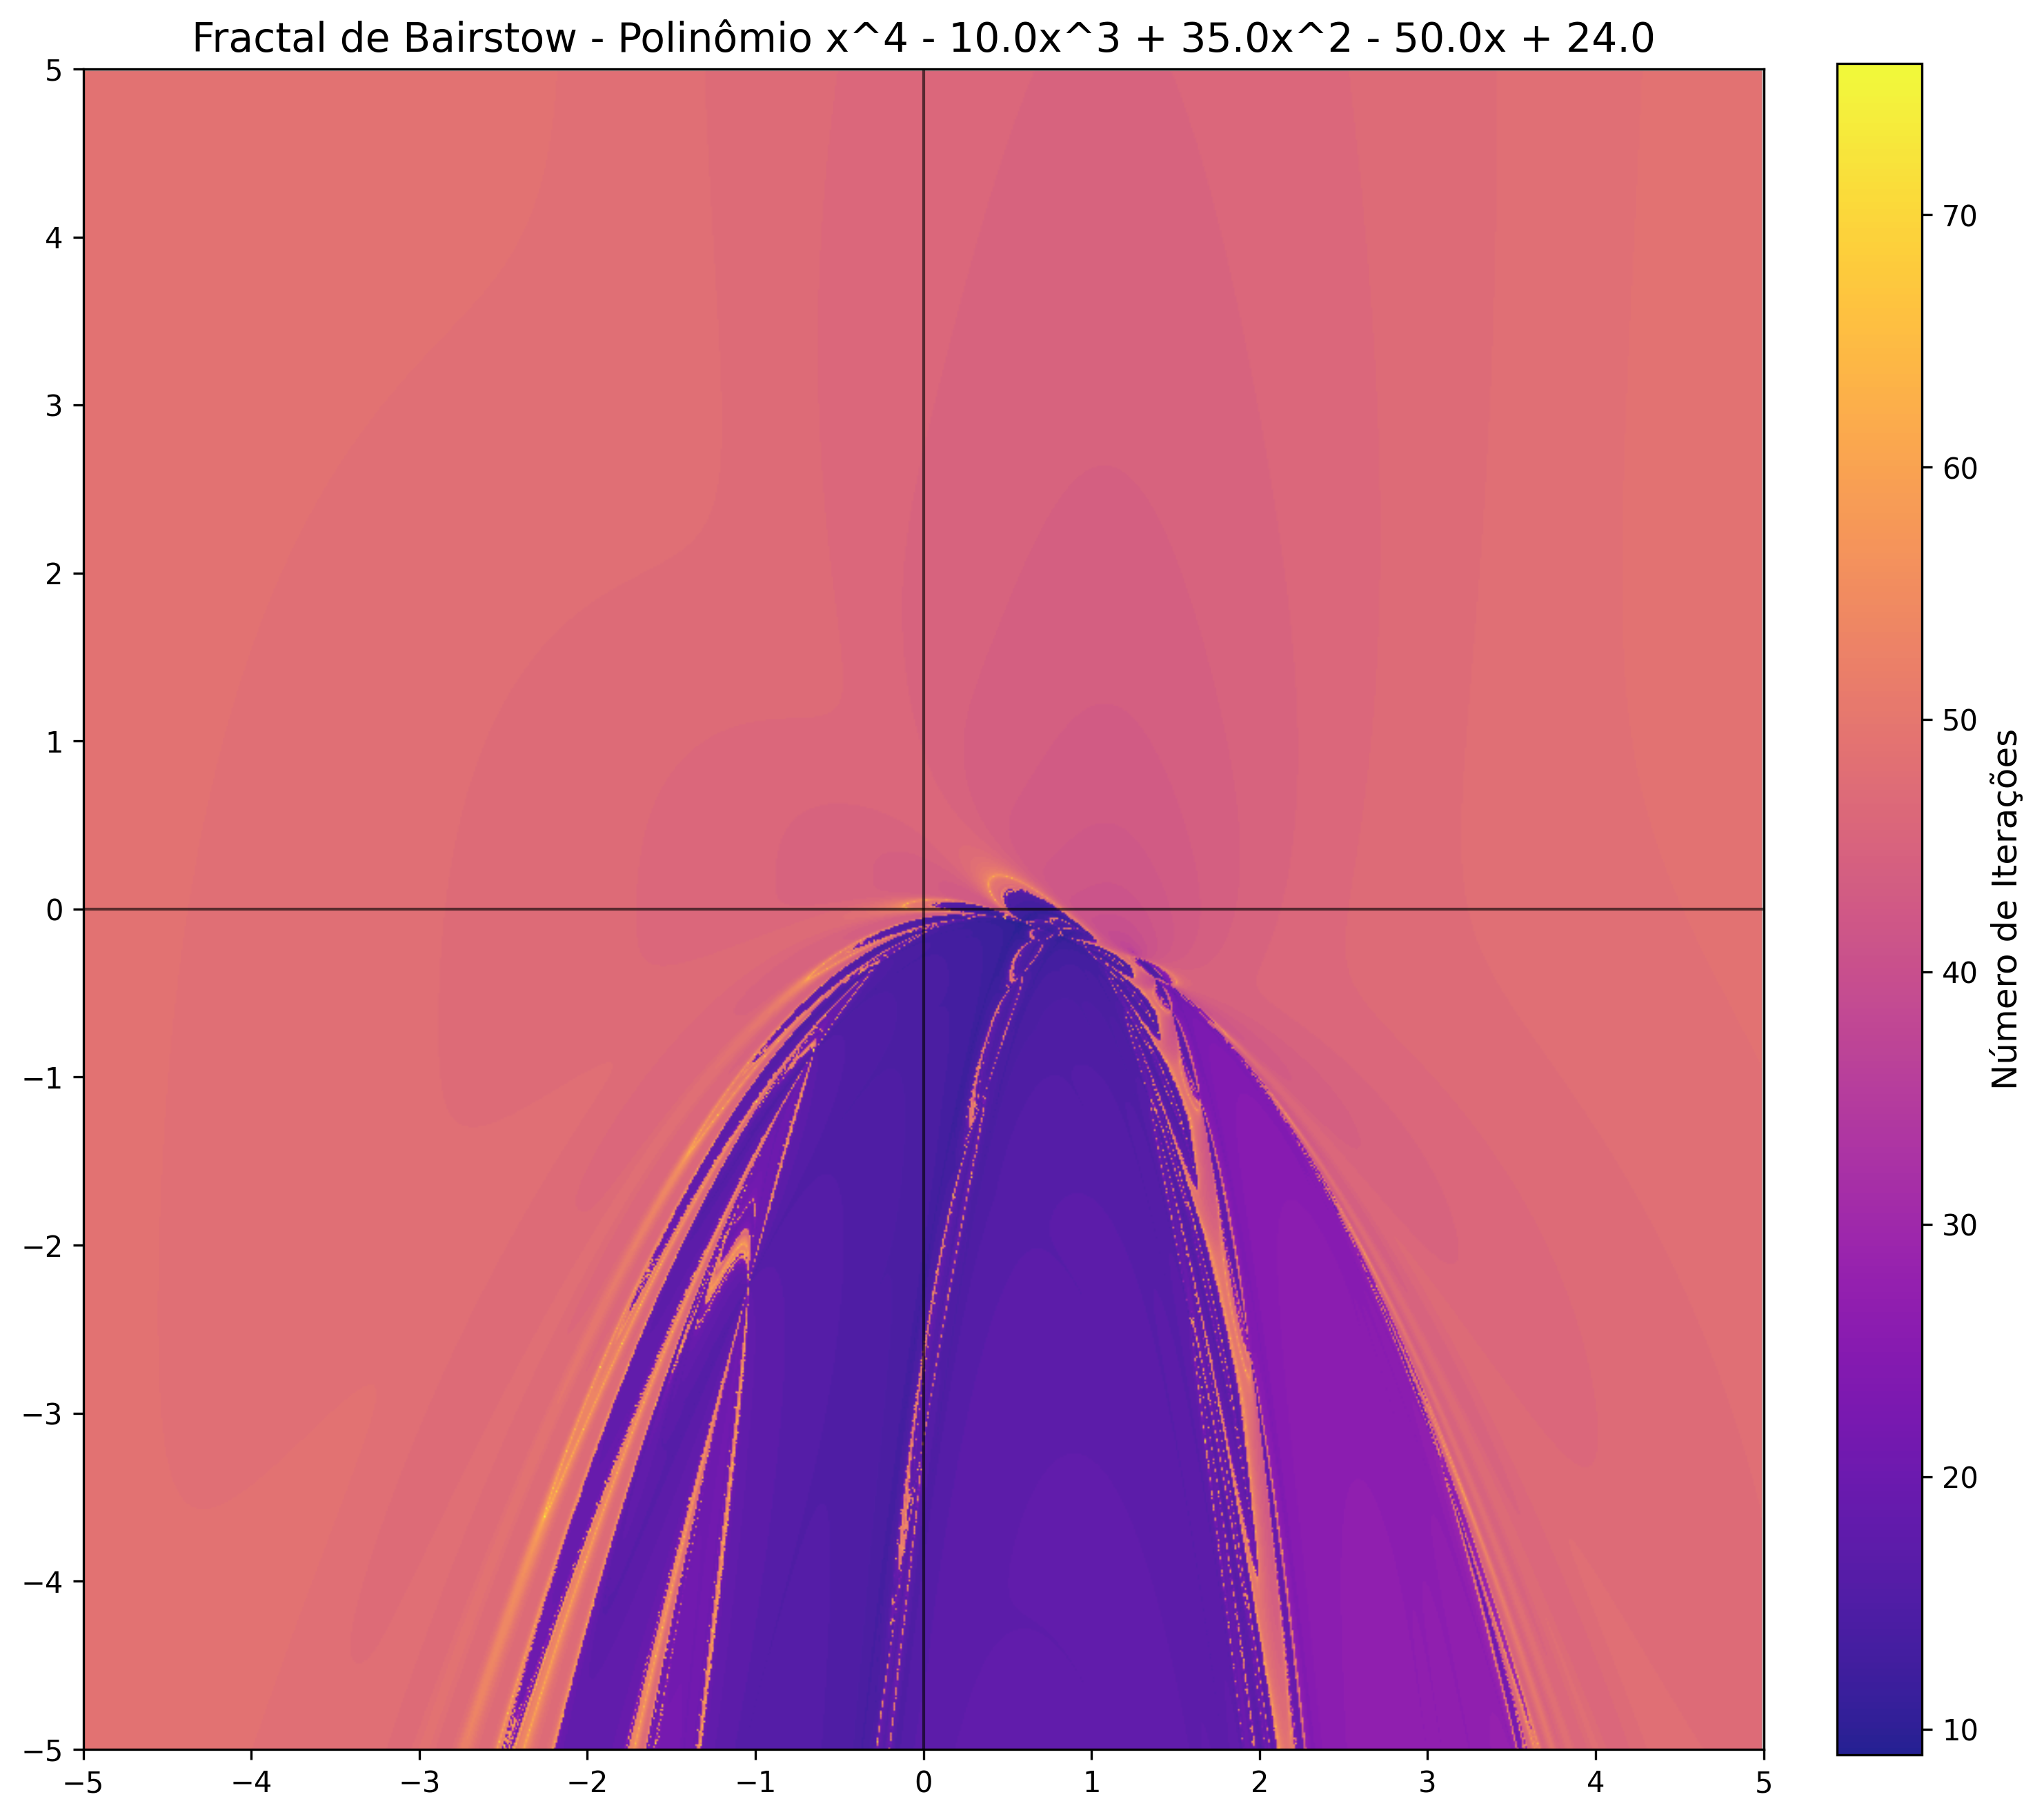
\includegraphics[width=0.8\textwidth]{img/f6.png}
\caption{Fractal de iterações para $x^4 - 10x^3 + 35x^2 - 50x + 24$.}
\end{figure}

\begin{figure}[H]
\centering
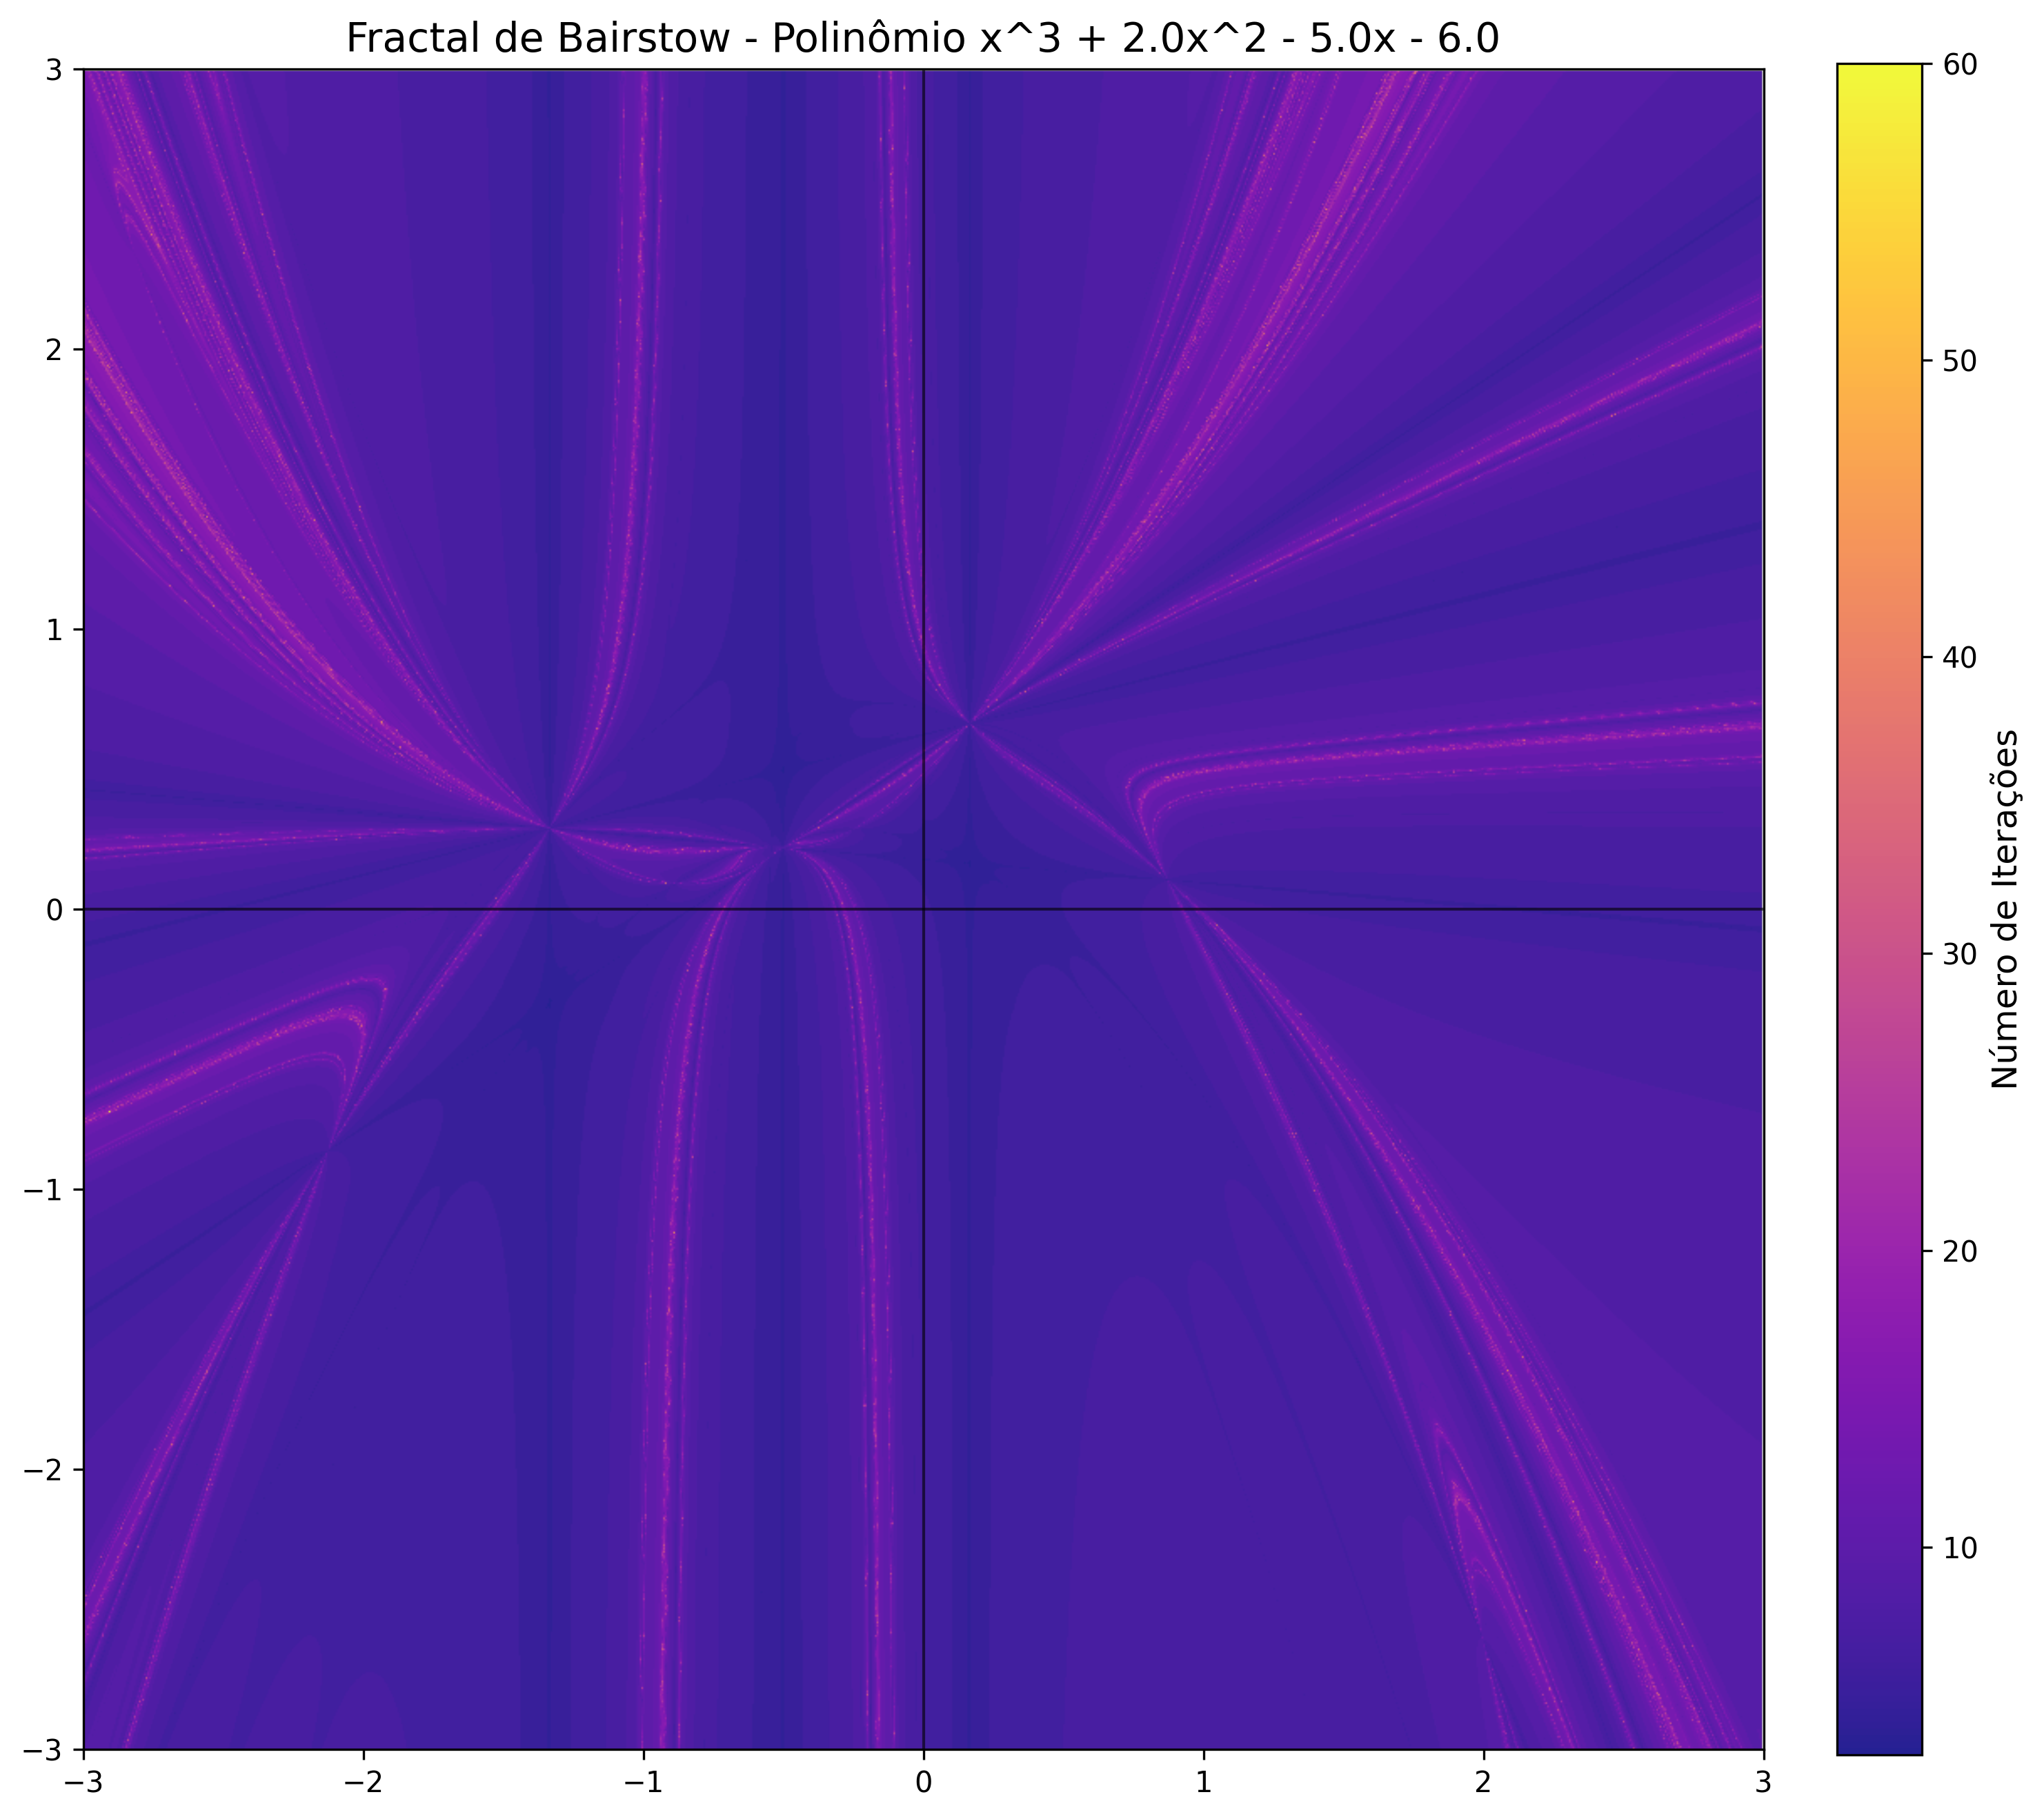
\includegraphics[width=0.8\textwidth]{img/f7.png}
\caption{Fractal de iterações para $x^3 + 2x^2 - 5x - 6$.}
\end{figure}

\begin{figure}[H]
\centering
\includegraphics[width=0.8\textwidth]{img/f9.png}
\caption{Fractal de iterações para $x^5 - 5x^4 + 5x^3 + 5x^2 - 6x$.}
\end{figure}

\begin{figure}[H]
\centering
\includegraphics[width=0.8\textwidth]{img/f10.png}
\caption{Fractal de iterações para $x^6 + 3x^5 - 3x^4 - 21x^3 + 18x^2 + 54x - 8$.}
\end{figure}

\begin{figure}[H]
\centering
\includegraphics[width=0.8\textwidth]{img/f11.png}
\caption{Fractal de iterações para $x^6 - 3x^4 + 3x^2 - 1$.}
\end{figure}

\begin{figure}[H]
\centering
\includegraphics[width=0.8\textwidth]{img/f13.png}
\caption{Fractal de iterações para $x^5 - 5x^4 + 4x^3 + 22x^2 - 21x - 18$.}
\end{figure}

Outros fractais podem ser gerados facilmente com diferentes configurações de polinômios e malhas.

\section{Conclusão}

O Programa 4 atendeu integralmente aos objetivos propostos, proporcionando:

\begin{itemize}
\item Uma implementação robusta e modular do Método de Bairstow;
\item Ferramentas de visualização (fractais) que elucidam o comportamento dinâmico do método;
\item Capacidade de exportação e análise dos dados de iteração;
\item Controle preciso da execução, mesmo em casos difíceis.
\end{itemize}

O estudo dos fractais gerados revelou a alta complexidade e sensibilidade do Método de Bairstow, tornando esta ferramenta não apenas prática para cálculo de raízes, mas também rica para investigação didática e teórica.

\end{document}